\chapter{Usage}\label{usage}

\section{Introduction}\label{intro}

BlasterSim simulates pneumatic and spring compressed gas guns with a \href{https://en.wikipedia.org/wiki/Lumped-element_model}{lumped parameter} model.

With BlasterSim, you simulate a foam dart blaster or any other compressed gas gun before building.
BlasterSim can also help answer hypothetical questions about an existing build, like whether performance will benefit from a particular change.
Optimal barrel length can be accurately calculated, avoiding inaccurate rules-of-thumb and tedious experiments with varying lengths of barrel.

This guide starts with the usage (\secref{usage}) and theory (\secref{theory}) of BlasterSim.
Later chapters include comparisons of BlasterSim against experimental measurements (\secref{validation}), details of how BlasterSim is tested otherwise (\secref{verification}), how to contribute to BlasterSim (\secref{dev}), and notes on developing BlasterSim (\secref{compiling}).

BlasterSim is under development and not yet feature-complete.

\section{Installation}\label{installation}

BlasterSim has no dependencies.
BlasterSim is written in Fortran 2018 and will run on any computer a modern Fortran compiler allows.

Obtain the latest BlasterSim binary from \url{http://trettel.us/blastersim/releases/}.
For Linux, this is blastersim-\gittag-linux-x86-64.tgz. % chktex 8
For Windows, this is blastersim-\gittag-windows-x86-64.zip. % chktex 8
For macOS, this is blastersim-\gittag-mac-x86-64.tgz. % chktex 8

The \texttt{blastersim} executable on Linux/macOS and the \texttt{blastersim.exe} executable on Windows can either be placed in the directory you want to run BlasterSim from or placed on your \texttt{PATH}.

See \secref{compiling} for instruction on how to compile BlasterSim from the source tarball or clone of the Git repository.

\section{Running BlasterSim and BlasterSim outputs}\label{running}

With BlasterSim placed on your \texttt{PATH}, you can run BlasterSim by typing \texttt{blastersim} in your terminal.
With BlasterSim placed in your current directory, you can run BlasterSim by typing \texttt{./blastersim} on Linux or \texttt{blastersim} on Windows.

The first command line argument is the input file.
For example, to run BlasterSim on input.nml, type \texttt{blastersim input.nml}.

If BlasterSim is run without an input file by running the \texttt{blastersim} by itself, BlasterSim will print a message containing information about how to run BlasterSim, the BlasterSim version, and debugging information:
\lstinputlisting[breaklines=true]{blastersim-out-1.txt}

If BlasterSim is on your \texttt{PATH}, you can run BlasterSim with an input file like \texttt{blastersim springer-example.nml} to simulate the blaster described in the input file.
If BlasterSim is placed in your current directory, you can run BlasterSim with an input file like \texttt{./blastersim springer-example.nml} on Linux or \texttt{blastersim springer-example.nml} on Windows.
Using the example input file in \secref{springer-example} returns the following:
\lstinputlisting[breaklines=true]{blastersim-out-2.txt}

After BlasterSim completes, a CSV spreadsheet with detailed data the simulation is written.
This spreadsheet can be opened in a spreadsheet program like Excel or any other program that supports CSV spreadsheets.
The name of the spreadsheet is determined by the optional \texttt{id} input variable.
If \texttt{id} is not provided, it takes the default value of \texttt{output}, so the spreadsheet is written to output.csv.
In the example in \secref{springer-example}, \texttt{id} was set to ``springer-example'', so the spreadsheet is written to springer-example.csv.

\section{BlasterSim inputs in general}\label{inputs-general}

BlasterSim uses Fortran namelist format input files.
Namelist files are broken into groups and variables.
A group starts with the \texttt{\&} symbol, then the name of the group, and contains one or more variables which themselves are the actual input data.
A group ends with the \texttt{/} symbol.
For example, in the example namelist input file below, see that \texttt{group1} group contains the variables \texttt{a}, \texttt{b}, and \texttt{c}.
\texttt{a} is an integer, \texttt{b} is a floating point number (decimal number), and \texttt{c} is a string (which must be quoted).
A namelist file can contain multiple groups.
The example below has two groups, \texttt{group1} and \texttt{group2}.
Comments can be added with the \texttt{!} symbol.
Comments can take up an entire line as in the \texttt{group1} namelist below, or be placed at the end of a line as in the \texttt{group2} namelist below.

\begin{lstlisting}
&group1
a = 0
b = -1.01
c = "string1"
! comment
/

&group2
x = 1
y = 2.05 ! comment
z = "string2"
/
\end{lstlisting}

For more details of the namelist format, refer to the Intel Fortran Compiler documentation~\cite{noauthor_namelist_2025}.

BlasterSim uses SI units in its input files and internally.
Support for other unit systems is not planned due to the complexity of supporting multiple unit systems.
Scientific notation can be used to appropriately scale inputs.
For example, instead of 13 mm being written as \texttt{0.013}, the user can write \texttt{13.0e-3}.

\section{Springer mode}\label{springer}
% TODO

As shown in \figref{springer time zero}, BlasterSim geometrically models the plunger tube and barrel are treated as cylindrical.
However, BlasterSim does not assume a sudden contraction exists between the plunger tube and barrel as shown by the figure.
That part of the figure is for illustration only.
The connection between the plunger tube and barrel can take any form.

% chktex-file 1 chktex-file 8

\tikzmath{
\dplunger     = 3;
\lplungertube = 5;
\dbarrel      = 1;
\lbarrel      = 6;
\ldead        = 1.5;
\ylowbarrel   = (\dplunger - \dbarrel)/2; 
\yhighbarrel  = \ylowbarrel + \dbarrel;
\xbarrelend   = \lplungertube + \ldead + \lbarrel;
\xbarrelstart = \lplungertube + \ldead;
\lproj        = 2;
\xproj        = \xbarrelstart + 1;
\xplungerheadstart = 1.5;
\lplungerhead      = 0.5;
\xplungerheadend   = \xplungerheadstart + \lplungerhead;
\ycenter = \dplunger/2;
\yfullspring = -\dplunger/2;
\yfullspringbelow = -7*\dplunger/8;
\yfullspringbelowbelow = -\dplunger;
\yfullspringabove = -\dplunger/4;
\halfyfullspringabove = -1*\dplunger/8;
\lfullspring = 7;
\ylbarrel = \ycenter + (\dplunger + \dbarrel)/4;
\xdead = \lplungertube + \ldead/2;
\xplungerheadunprimed = \lplungertube - \lplungerhead;
\yxz = \ycenter - (\dplunger + \dbarrel)/4;
\xdbarrel  = \xbarrelend - 1;
\xdplunger = \xplungerheadend + 1.0;
}

\begin{figure}
\centering
\begin{tikzpicture}
\draw[thick] (\xbarrelend, \yhighbarrel) -- (\lplungertube, \yhighbarrel) -- (\lplungertube, \dplunger) -- (0, \dplunger) -- (0, 0)         -- (\lplungertube, 0) -- (\lplungertube, \ylowbarrel) -- (\xbarrelend, \ylowbarrel);

\draw[thick,dashed] (\lplungertube, \ylowbarrel) -- (\lplungertube, \yhighbarrel);

\fill[fill=gray,draw=black,thick] (\xproj, \ylowbarrel) rectangle ++(\lproj, \dbarrel);

\fill[fill=gray,draw=black,thick] (\xplungerheadstart, 0) rectangle ++(\lplungerhead, \dplunger);

\tikzstyle{spring}=[thick,decorate,decoration={coil,amplitude=20,segment length=4pt}] % `zigzag` doesn't work right in LaTeXML, but `coil` does
\draw[spring] (0, \ycenter) -- (\xplungerheadstart, \ycenter);

\draw[<->,thick,fill=white] (\xbarrelstart, \ylbarrel) -- node[above] {$l_\text{travel}$} (\xbarrelend, \ylbarrel); % `fill=white` added to make the text fully visible in LaTeXML
\draw[thick,dashed] (\xbarrelend, \yhighbarrel) -- (\xbarrelend, \dplunger);

\node[draw=white] at (\xdead, \ycenter) {$V_\text{dead}$}; % `draw=white` added to make the text fully visible in LaTeXML

\draw[<->,thick] (\xplungerheadend, \halfyfullspringabove) -- node[below] {$y$} (\lplungertube, \halfyfullspringabove);
\draw[thick,dashed] (\lplungertube, \yfullspringabove) -- (\lplungertube, 0);
\draw[thick,dashed] (\xplungerheadend, \yfullspringabove) -- (\xplungerheadend, 0);

\draw[<->,thick] (\lplungertube, \ylbarrel) -- node[above] {$x_\text{0}$} (\xbarrelstart, \ylbarrel);
\draw[thick,dashed] (\xbarrelstart, \ylowbarrel) -- (\xbarrelstart, \dplunger);

\draw[<->,thick] (\lplungertube, \yxz) -- node[below] {$x$} (\xproj, \yxz);
\draw[thick,dashed] (\xproj, 0) -- (\xproj, \ylowbarrel);

\draw[<->,thick] (\xdbarrel, \ylowbarrel) -- node[right] {$d_\text{barrel}$} (\xdbarrel, \yhighbarrel);

\draw[<->,thick] (\xdplunger, \dplunger) -- node[right] {$d_\text{plunger}$} (\xdplunger, 0);
\end{tikzpicture}
\caption{Model spring blaster at arbitrary time as represented in BlasterSim.\label{fig:springer time zero}}
\end{figure}

\begin{figure}
\centering
\begin{tikzpicture}
\tikzstyle{spring_unprimed}=[thick,decorate,decoration={coil,amplitude=20,segment length=18pt}]
\tikzstyle{spring_full}=[thick,decorate,decoration={coil,amplitude=20,segment length=30pt}]
\draw[thick] (\xbarrelend, \yhighbarrel) -- (\lplungertube, \yhighbarrel) -- (\lplungertube, \dplunger) -- (0, \dplunger) -- (0, 0)         -- (\lplungertube, 0) -- (\lplungertube, \ylowbarrel) -- (\xbarrelend, \ylowbarrel);

\fill[fill=gray,draw=black,thick] (\xplungerheadunprimed, 0) rectangle ++(\lplungerhead, \dplunger);

\draw[spring_unprimed] (0, \ycenter) -- (\xplungerheadunprimed, \ycenter);

\draw[spring_full] (0, \yfullspring) -- (\lfullspring, \yfullspring); % has a long straight line segment in LaTeXML for some reason
\draw[<->,thick] (0, \yfullspringbelow) -- node[below] {$l_\text{spring}$} (\lfullspring, \yfullspringbelow);
\draw[thick,dashed] (0, \yfullspringbelowbelow) -- (0, 0);
\draw[thick,dashed] (\lfullspring, \yfullspringbelowbelow) -- (\lfullspring, 0);

\draw[<->,thick] (\lfullspring, \halfyfullspringabove) -- node[above] {$\Delta_\text{pre}$} (\xplungerheadunprimed, \halfyfullspringabove);
\draw[thick,dashed] (\xplungerheadunprimed, \yfullspringabove) -- (\xplungerheadunprimed, 0);
\end{tikzpicture}
\caption{Unprimed ($y = 0$) model spring blaster as represented in BlasterSim to show spring precompression.\label{fig:springer unprimed}}
\end{figure}

\begin{figure}
\centering
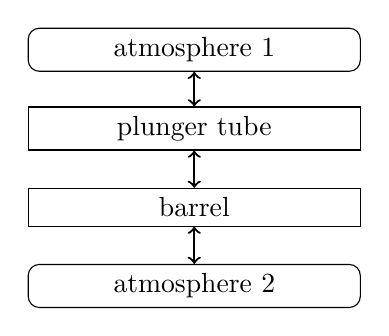
\begin{tikzpicture}
\tikzstyle{cv}       = [rectangle, minimum width=12em, text centered, draw=black]
\tikzstyle{cv_const} = [rectangle, rounded corners, minimum width=12em, text centered, draw=black]
\tikzstyle{arrow}    = [thick, <->]

\node (atm1)         [cv_const]                  {atmosphere~1};
\node (plunger tube) [cv, below of=atm1]         {plunger~tube};
\node (barrel)       [cv, below of=plunger tube] {barrel};
\node (atm2)         [cv_const, below of=barrel] {atmosphere~2};

\draw [arrow] (atm1)         -- (plunger tube);
\draw [arrow] (plunger tube) -- (barrel);
\draw [arrow] (barrel)       -- (atm2);
\end{tikzpicture}
\caption{Abstract connected control volume view of a springer blaster.\label{fig:springer control volumes}}
\end{figure}


\subsection{\texttt{springer} namelist group variables}\label{springer-namelist}

The following variables are in the springer namelist group.
If there is a corresponding typeset variable, the notation for that variable is also listed.

\input{defaults.tex}
\input{geninput_springer.tex}

\subsection{Example springer input file}\label{springer-example}
% TODO: Go through file and explain what it means.

\lstinputlisting{springer-example.nml}

\section{Pneumatic mode}\label{pneumatic}
% TODO

\subsection{\texttt{pneumatic} namelist group variables}\label{pneumatic-namelist}
%TODO

\subsection{Example pneumatic input file}\label{pneumatic-example}
% TODO: Add example
% TODO: Go through file and explain what it means.

\section{BlasterSim internal model}\label{internal-model}
% TODO

Internally, BlasterSim simulate blasters using control volumes with arbitrary flow connections between control volumes.
This allows BlasterSim to simulates spring and pneumatic blasters with the same core simulation code. This also allows simulating more atypical blasters without major code changes.

This section describes the internal model in an abstract way.
See \secref{interior-ballistics} for details on the specific equations solved.
